\documentclass[english]{tktltiki}
\usepackage[pdftex]{graphicx}
\usepackage{subfigure}
\usepackage{url}
\usepackage{algpseudocode}
\usepackage{amssymb}
\usepackage{amsmath}
\usepackage{graphicx}
\usepackage{algorithmicx}
\usepackage[Algorithm,ruled]{algorithm}
\usepackage{float}


\DeclareMathOperator*{\argmax}{arg\,max}
\begin{document}
%\doublespacing
%\singlespacing
\onehalfspacing

\title{Influence Maximization in Large Scale Graphs}
\author{Behrouz Derakhshan}
\date{\today}

\maketitle

\numberofpagesinformation{\numberofpages\ pages + \numberofappendixpages\ appendices}
\classification{\protect{\ \\
\textbf{Information systems --> Graph-based database models},\\
\textbf{Information systems --> MapReduce-based systems}}}

\keywords{Graph, Influence maximization, Big Data, Hadoop, Spark}

\begin{abstract}

Maximizing influence in graphs, typically applied to Social Networks, is the problem of finding a set of nodes that have the highest overall influence on the entire graph. In marketing domain for example, it is used to find a set of people who have the highest influence on their local communities and instead of blindly marketing a product to a large group of users, only those users are selected and the product is marketed to them, they will in turn help spreading the word to other people around them. The problem has been studied extensively, and several state of the art methods have been proposed. But they all suffer from scalability issues. Even on small graphs, current methods take an extremely long amount of time. Over the past two decades, collection of data has become easier and very common mostly because advancements in hardware and software technologies and the existence of World Wide Web. To over come issues related to big data sets, large scale data processing platforms have been developed over the past couple of years to tackle scalability issues of problems similar to influence maximization. Most notably are two frameworks called Hadoop and Spark that contain many features for simple data processing, machine learning and graph processing. In this thesis work, some of the current influence maximization algorithms are implemented in these two frameworks, some new methods are proposed and experiments on graphs of different sizes are performed and the results are reported. 

\end{abstract}

\mytableofcontents

\section{Introduction}
The term graph, first used by mathematician J. J. Sylvester, is a representation of set of interconnected objects. Typically, in a graph the interconnected components are called vertices, and the links that are connecting them are called edges. Graph theory, is the field of mathematics that studies graphs and since its introduction, it has been used extensively, in many branches of science. In computer science, graphs can represents, networks of computers, websites and the communication between them. In Chemistry and Physics, graphs are used to model the atoms and molecules and their interactions. Graphs components, can also carry extra information, for example the edges can carry weight which can quantify or qualify the connection between two nodes. For example in a graph that represent geographical locations, where vertices (nodes) represent places, the edges represent the length between the locations. \\
Over the past two decades with the introduction of social network, it has been use extensively to model the interactions between people belonging to a social network. One application that has been studied in social network or in graphs in general is the spread of information between nodes, based on the structure of the graph and the edge weights. In medicine and biology it has been used to find the spread of a disease either to find the initial person who contracted the disease or finding key vertices that could amplify the spread and by identifying those nodes further spread of the disease can be avoided. In social network, it has direct application, sociologists have applied influence maximization methods to study the spread of information between people in a network, and how individual can affect each other. Marketing is another applications of influence maximization.  Domingo and Richardson \cite{domingo01} were the first to study the spread of information in networks of people. Being generally referred to as the \textit{Word Of Mouth} phenomena, it shows how different people influence each others opinion, even though there is no direct relationship between them. Prior to them, most of the research in marketing were to maximize the profitability of single customers, and disregarding the effect they have on the whole network. Domingos and Richardson proposed a method to estimate the value of customers in term of the network and how much a customer will increase profitability of the whole market if an item is advertised to him/her. Kempe et al. \cite{kempe03} formally defined the problem of \textit{Influence Maximization}. By studying how influence is propagated under two models; \textit{Independent Cascade} and \textit{Linear Threshold} models, they defined the problem of Influence Maximization as finding an initial set of people, that will influence the most number of people under either models. They have also proved that the problem of \textit{Maximizing Influence} is a \textbf{NP-hard} problem, the solution they proposed involves a greedy algorithm that approximates a solution which is guaranteed to be within 63\%  of the optimal solution. Since its introduction, Influence maximization has been studied extensively, many has tried to optimize and speed up the original greedy method and several others have tried to propose different methods for finding the solution. The main issue with the greedy method is in the objective function and how it is calculated. Since there's no exact was of estimating the spread of an initial set, several simulations are run using either of the propagation models, using the same initial set and the result is the average of all the simulations. To guarantee an accurate solution, many thousands of simulations have to be run, and due to the nature of the problem, even on small to medium size graphs, this is highly inefficient. In the next sections, the details of the algorithm and its deficiencies when it comes to speed and scalability are discussed. \\
Over the past couple of years, with introduction of social networks, online web stores and other websites that engages users, massive amount of data and information are being gathered everyday. Social networks such as Facebook and Twitter has hundreds of millions of active users, that are interacting with each other daily. Web stores such as Amazon, sells products to millions of users, most of which have friends and acquaintances buying the same or similar products and are constantly being influenced by their decision on the specific products. Even customers that have never met each other usually have access to each others review of these products. These massive amount of information are usually modeled as network of people and analyzing them  has been proven to be an extremely difficult tasks. A field of computer science has emerged recently that focus on building systems, methods and algorithms that deal with massive amount of data. Generally referred to as to as the field of \textbf{Big Data}, it involves, platforms that can analyze data in such amount that are impossible for a normal computer to analyze. Probably the most notable framework that is used widely nowadays is called \textbf{Hadoop}. Hadoop is open source project that is based on Google's MapReduce framework. Originally developed to include the map reduce framework and a file system capable of catering terabytes or even petabytes of data reliably and efficiently, called \textit{Hadoop Distributed File System(HDFS)}, Hadoop has since improved to include many different frameworks, include different tools and systems each capable of analyzing and processing large scales. Currently, Hadoop is referred to a set of big data technologies, each with unique use cases that works very well together. One of recent additions to the Hadoop suite is \textit{Spark}, a framework capable of processing massive amount of data, that approaches the processing of data differently from the traditional map reduce framework. \\
As discussed before graphs are powerful modeling frameworks, capable of storing many different information about objects, but modeling data of this volume cannot be done using conventional graph modeling framework. Using these and other similar frameworks, many graph processing tools and applications are built which utilizes the mechanism of these frameworks to process graphs of millions or billion of nodes and trillions of edges. \\
Two notable graph processing framework based on Hadoop's map reduce and Spark are :
\begin{itemize}
\item 
Giraph which is open source project by on Google's Pregel framework. It is built on top of Hadoop's map reduce
\item 
GraphX is open source project built on top of Spark
\end{itemize}
Many other graph frameworks for processing large scale data exists, but the core difference between most of them and Giraph and GraphX are; first of all both Giraph and GraphX are open source, so developers have access to the code and can modify and observe the code to better understand and made changes that suites their needs. In the next sections, these frameworks are more closely studied and their features are presented in details. \\
The aim of this thesis is to study in detail the problem of influence maximization in social networks, current state of art algorithm for the problem. Disadvantages of the methods, specially regarding the scalability are discussed and different methods are proposed to solve the issue, using large scale graph processing system. \\
The rest of this document is organized as follow; in section 2 Big Data framework, their history and the current state are discussed, two of the very common frameworks, i.e. Hadoop and Spark are studied in detail. In section 3, different large scale graph processing frameworks are compared and Giraph which is based on Hadoop's MapReduce and GraphX which is based on Spark are explained in great detail. Section 4, contains the history of influence maximization problem, different methods that have been proposed so far, their advantages and disadvantages are discussed. In section 5, scalability issue of influence maximization is studied, and several methods either novel or based on previous methods are proposed and the implementation details are discussed. Section 6 concludes the thesis, and future works, problems that were not covered in the document are discussed


\newpage

\section{Influence Maximization}
Effective marketing and advertisement methods has been a major application of Knowledge Discovery and Data mining. Prior to \cite{domingo01} the focus has always been on direct marketing. Contrary to traditional mass marketing, where a product was marketed to all the customer, in direct marketing the goal is find the most potential and profitable costumers.  One example is \textbf{Recommendation Systems} which based on users previous purchasing habits will recommend new items. While direct marketing is a great tool for increasing the profit, it only targets individuals and disregards the relationship between users. People's decision in purchasing an item is not only influenced by the product itself, but also by friends, colleagues and acquaintances. With introduction of Internet and Social networks, gathering information about users became easier and more feasible. Social networks nowadays contains information about millions of people, they also contain information related to people's relationship with each other. Utilizing these information, can make marketing more profitable, by targeting people that are more likely to promote the product to their acquaintances. 
\cite{domingo01} discussed the use case of influence maximization in marketing, calling it \textbf{Viral Marketing}. By modeling a market as a social network consisting of users and products. In such a network, probability of users buying products only depends on the product itself, the neighbors of the user and the set of marketing actions being applied to the network. Hence the market can be formulated as join probability distribution. 
Through these a function was devised that calculates the global lift in profit given a marketing action was applied to some users. Starting from an initial configuration, using different optimization algorithms a local maxima for the function can be reached. Hence the problem of influence maximization can be formulated as follows. \\ \\
\textit{Given a size $k$ for the initial seeds, find the set of nodes $A$ that maximizes the function $f$ which is the size of spread through out the network . }\\ \\
They experimented on a collaborative filtering data set (MovieLenz) in which users have rated a list of movies. They have first constructed the network with the user ratings, by choosing similar users(calculating the Pearson correlation coefficient of users) as neighbors . They have performed experiments on the data set and compared their method with mass marketing and direct marketing. Their method has increased the profit the most. Due to non-linearly of the model, it did not scale well for bigger size networks, hence they have proposed a new linear model \cite{domingo02}. Not only the new model decreased the computation time, they simplified equation for calculating the network value of customers, made it easier to incorporate more complex marketing action. They have experimented with Epinions \footnote{http://www.epinions.com/}data set. Which is a website where users can rate items. It also has a feature called trusted users, where each user can select many other users as trusted sources of reviews. Domingo et .al, hence, applied their model to the dataset, by considering trusted users of a user his neighbors. Their experiments showed that a continuous marketing action (a marketing action that can have unlimited values, such as a discount) performs much better than boolean marketing actions (one that can either be true or false, such whether or not a discount should be given to a user with no regards for the amount of the discount).  
\subsection{Information Diffusion Models}
With introduction of Social Networks, the topic of information diffusion has gain interest in research community. Information diffusion models describe how information and data are being propagated and transferred in social networks. Information diffusion is not only limited to social networks, for many years the topic has been studied to better understand for example how a disease is being spread among people or how contaminated water would affect a water pipe network. In influence maximization Kempe et .al \cite{kempe03}  studied two important information diffusion models.
\begin{itemize}

\item Linear Threshold Model :\\
Consider a directed graph G representing a social network, and individual nodes being either active or non-active. Inactive nodes may become active as more of their neighbors become active but the reverse is not possible. In \textit{Linear Threshold Model} each node $v$ is influenced by each of their neighbors $w$ according to a weight $b_{v,w}$ such that $\sum \nolimits_{w \, neighbor \, of \, v} b_{v,w} < 1$ . The diffusion process hence is as follows; each node $v$ will randomly chose a weight threshold $0 < \theta_v<1 $, this value determines tendency of node $v$ to become active. Starting from the initial seed set, in each iteration for each node if the sum of the weights of its active neighbors is greater than the threshold then the node will become active, i.e. $\sum \nolimits_{w \, active neighbor \, of \, v} b_{v,w}  \geq \theta_v $. The process is deterministic however since $\theta_v$ is chosen at random, it shows our lack of knowledge of their values. This process continues until no new nodes become active.

\item Independent Cascade Model :\\ 
 \textit{Independent Cascade Models} is a stochastic undeterministic process. Same as \textit{Linear Threshold Model}, it starts with an initial set of seeds, and in each time step $t$ every active node will try only once to activate all of its neighbors, the probability of a node $v$ activating one of its neighbors $w$ is define by a system property $p_{v,w}$. The process continues until no more new node can become active. Every node will try to activate its neighbors independently of other nodes, and if during one time step, a node $v$ first becomes active by node $u$ the rest of $v$'s neighbors can skip the activation process. In that sense the ordering of which nodes should to activate their neighbors first does not matter and it will not affect the final result.
\end{itemize}
Based on \textit{IC} different models have been also discussed, such as \textit{Weighted Cascade} which is similar to \textit{IC} with the exception of the activation probability. Where in \textit{IC} it is defined as a global property, in \textit{Weighted Cascade} each edge from $u$ to $v$ is assigned the probability $1/d_v$, where $d_v$ is the degree of vertex $v$. The probability for edges in weighted methods can be calculated in different ways, in fact finding the influence of nodes on each other is another research area in influence maximization and it is briefly explained in \ref{subsec:learninginfprob} .

\subsection{Influence Maximization Problem}
Kempe et .al \cite{kempe03} were the first to formulate Influence maximization as an optimization problem and prove that the problem is NP-complete. By studying how influence propagates through networks, they discussed two diffusion models \textit{Linear Threshold Model} and \textit{Independent Cascade Model}. They have formally expressed Domingos and Richardson's \cite{domingo01} optimization problem in the context of the above models. Both models involve an initial set of nodes $A$, the influence of a set $\sigma (A)$ is then defined as the number of nodes at the end of the process. Finding the optimal set is NP-hard but they proposed an approximation algorithm for the problem which guarantees the solution to be a factor of $(1 - 1/ \mathrm{e} - \varepsilon)$ of the optimal solution (slightly better that 63\%). 
Approximate solution for these models is developed based on \textit{submodular functions} \cite{nemhauser78}.
A function $f$ is \textit{submodular} if it satisfies a natural ''diminishing returns'' property. It means the marginal gain of adding a node $v$ to a set $A$ is always greater than or equal than adding $v$ to a super set of $A$ . 
\begin{center}
$f(A \cup \{v\}) - f(A) \geq f(S \cup \{v\}) - f(S)$, where $A \subseteq S$
\end{center}
The greedy algorithm proposed by Kempe i \cite{kempe03} is described in Algorithm \ref{alg:KempeInfMax1}. 
\begin{algorithm}[ht!]
\floatname{algorithm}{Algorithm}
\caption{Greedy Algorithm}
\label{alg:KempeInfMax1}
\begin{algorithmic}
\Require k,G(V,E)
\State S = $\emptyset$
\For {i = 1 to k}
	\For {every $v \in V$ and $v \notin S$}
		\State $\delta_v = \sigma(v)$
	\EndFor
	\State $v^* = \argmax_v \{\delta_v\}$
	\State $S = S \cup v^*$
\EndFor
\end{algorithmic}
\end{algorithm}
\\
They have run experiments on co-authorship in physics theory section of arXiv \footnote{www.arxiv.org}. The results show that their greedy algorithm performs better that other methods such as random selection, high-degree or central nodes .
Both in estimating the spread and also in the greedy method, $\sigma (S)$ has to be calculated, but both of the propagation models are non-deterministic. To overcome this, the model is run many times (10000 times) and the spread is the average of all the runs. The nature of the spread function makes the algorithm highly non scalable. Even on medium sized graphs running the simulation thousands of time will take a lot of time, but on the other hand a good solution is only guaranteed if the simulation is run many times. From Algorithm \ref{alg:KempeInfMax1} it can be observed that $\sigma(v)$ is run for every node in every iteration, this will greatly affect the performance of the greedy method.
Leskovec et .al \cite{leskovec07}  in their Cost effective outbreak detection in networks, took upon the task of optimizing the greedy method used in propagation in graph networks. Although they did not work on solving the problem of maximizing influence they have proven their method can be adapted to the problem of maximizing the influence using the greedy algorithm. They studied two problems from different domains which share similarities. The first problem is find the best placement of sensors in a water network, so that contaminated water can be detected as quickly as possible. The other problem is blog network, which is to find blogs that contains the maximum amount of news that cascades from different sources in shortest possible time. Their advanced greedy method, called CELF, utilizes the submodularity of the objective function, which reduces the amount of computation needed to be made in each iteration. Their method is 700 times faster than a simple greedy function. 
Their observation is that, if A is subset of B, the marginal gain of adding a node to B is always less than or equal to the marginal gain of the adding the same node to A. Hence instead of recomputing the gain for all the node in each iteration, we can go through the nodes in decreasing order of their spread and recompute their values, the change is usually very small and most of the time the value on top of the list stays on top. Algorithm \ref{alg:celf} describes CELF method .
\begin{algorithm}[ht!]
\floatname{algorithm}{Algorithm}
\caption{CELF}
\label{alg:celf}
\begin{algorithmic}
\Require G(V,E) : Graph G, with Vertex set V and Edge set E
\Require k: Initial Set Size
\State S = $\emptyset$
\For {i = 1 to k}
	\State set $\delta_v = \sigma(v)$ for $v \in V \setminus S$
	\While {TRUE do}
		\State $u =  \argmax_{v \in V \setminus S}\delta_v$ 
		\If {$I(u) = 0$}
			\State $\delta_u = \sigma( S \cup \{u\}) - \sigma(S)$
			\State $I(u)=1$
		\EndIf
		\If {$\delta_u \geq max_{v \in V \setminus (S \cup \{u\})}\delta_v$}
			\State $S = S \cup \{u\}$
			\State break
		\EndIf
	\EndWhile 
\EndFor
\State Output $S$
\end{algorithmic}
\end{algorithm}
As can be seen from the algorithm description, the difference between CELF and the normal Greedy method, is that in CELF, $\delta(v)$ is pre-calculated for all the vertices first, then starting from the biggest value, in each iteration $\delta(u)$ is recalculated for vertex $u$ if the value is still higher than the next vertex in the list, then node $u$ is added to $S$ otherwise the next vertex is chosen. As in the previous algorithm, $\sigma(v)$ is the expected spread of the node $v$ under the \textit{Independent Cascade model}.
\cite{chen09}proposed several different methods for solving the problem of Influence Maximization. The first group of algorithms, were improvement upon Kempe \cite{kempe03} and Leskovec \cite{leskovec07} greedy method. In their greedy method, they have modified the simulation process. Instead of trying to activate nodes based on the edge probability one by one, they have first created a new Graph $G'$ which is sampled from the original graph based on the edge probability. Now the process of estimating the spread of initial set $S$ is just finding the number of reachable nodes in $G'$ from $S$, this process is repeated many times and the result is the average for all of the $G'$ sampled Graphs. Although this method is much faster than the original greedy method, it cannot compete with Leskovec \cite{leskovec07} CELF method, since in their method only in the first iteration the spread for all the nodes are calculated and from the second iteration onward, due to submodularity only the spread for a few of the nodes are recalculated. Hence, they have combined their new Greedy method with CELF, where in the first iteration they use the sample graphs to calculate the spread and in the following iterations CELF is used. The second class of algorithms they have proposed are a set of heuristics for finding the set of the seed that maximizes the influence. Prior to their work, heuristics have been considered inferior to the Greedy method and while that is true for many of the heuristics, such as degree, random, distance and etc., their proposed heuristic called \textit{DegreeDiscountIC}managed to achieve almost the same spread with the greedy method while outperforming the greedy methods by orders of magnitude. Details of the algorithm \textit{DegreeDiscountIC} is explained in section 3 \ref{subsec:degreediscount}.

Other notable heuristic method is of Saito and Kimura \cite{kimura06}. They have investigated the scalability issue of IC model simulations. They have argued that the current simulation model in ICM requires many iterations and each iteration took a lot of processing time and power. They have proposed two natural special cases of the ICM such that a good estimate of this quantity can be efficiently computed. They define the Shortest-Path Model(SPM) which is a special case of the ICM such that each node $v$has the chance to become active only at step = $d(A,v)$ , where if $A$ is the initial set, $d(A,v)$ is the distance of $A$ to node $v$. This means that each node is activated only through the shortest paths from the initial active set. The other model they have proposed named SP1M, which is each node v has the chance to become active only at steps t = d(A,v) and t =d(A,v) + 1. Through these two models they have proposed methods for calculating the spread of an initial set A. They have proved that the result achieved using this method is also within a bound of the best solution. In their experiments, they have assigned a uniform probably to each edge with two different values p = 0.1 and p =0.01. The experiments showed that the estimation of the spread for ICM increases as p increases while the processing times for the SPM and SP1M hardly change. 

\cite{cheng13} Have addressed both the accuracy and scalability of the solutions using the greedy methods. They have pointed out the main bottle neck in methods based on \cite{kempe03} are in the Monte Carlo simulation steps. They have proven that the objective function is not entirely sub-modular due to the randomness in the simulations, and hence to compensate for that many Monte Carlo simulations have to be run in each step of the algorithm which greatly reduces the performance.
They proposed a new method called StaticGreedy which computes a series of snapshots at the beginning of the algorithm and reuses those for every step of the greedy algorithm.  They have defined two terms, snapshots and simulations which can be both used for the Monte Carlo simulations. \\
\begin{itemize}
\item 
Simulation : The influence spread is obtained by directly simulating the random process of diffusion triggered by a given seed set $S$.
\item
Snapshot : According to the characteristic of IC(Independent Cascade) model, whether u successfully activates v depends only on $p(u,v)$. Hence prior to the main algorithm a Graph $G'=(V,E')$, which is a subgraph of G where an edge $E(u,v)$ is remained with the probability $p(u,v)$ and deleted otherwise. 
\end{itemize}
Before the main steps of the algorithm many snapshots are produced and averaged to estimate the spread function. 
Have StaticGreedy algorithm here :\\
1. Static snapshots \\
2. Greedy selection \\

Two main difference between this method and the previous ones are :
\begin{itemize}
\item
Monte Carlo simulations are conducted on static snapshots, which are sampled before the greedy process of selecting seed nodes
\item
The same set of snapshots are reused in every iteration to estimate the influence spread $I(S)$, which explains the meaning of ''static''
\end{itemize}

They have performed experiment and compared their methods with the normal Greedy methods. None of the other greedy methods are any match with StaticGreedy in terms of speed and scalability. \\
\begin{algorithm}[ht!]
\floatname{algorithm}{Algorithm}
\caption{UBLF}
\label{alg:ublf}
\begin{algorithmic}
\Require G(V,E) : Graph G, with Vertex set V and Edge set E
\Require PP : Propagation probability matrix of G
\Require k: Initial Set Size
\State S = $\emptyset$ and $\delta = (I - PP)^{-1} .1$ 
\For {i = 1 to k}
	\State set $I(v) = 0$ for $v \in V \setminus S$
	\While {TRUE do}
		\State $u =  \argmax_{v \in V \setminus S}\delta_v$ 
		\If {$I(u) = 0$}
			\State $\delta_u = \sigma( S \cup \{u\}) - \sigma(S)$
			\State $I(u)=1$
		\EndIf
		\If {$\delta_u \geq max_{v \in V \setminus (S \cup \{u\})}\delta_v$}
			\State $S = S \cup \{u\}$
			\State break
		\EndIf
	\EndWhile 
\EndFor
\State Output $S$
\end{algorithmic}
\end{algorithm}
Zhuo et .al \cite{zhuo13} propsed a new Greedy algorithm called \textit{Upper Bound based Lazy Forward algorithm(UBLF)}. They have tried to bound the number of Monte Carlo simulation calls, similar to \cite{leskovec07}'s CELF algorithm. CELF, increased speed of the original algorithm by a factor 700 on average case, the bottleneck in the algorithm is the however in the first iteration, where for each vertex the spread has to be estimated, that means Monte Carlo simulations have to be run for all the vertices in the first iteration, and it was argued before that, while that is reasonably fast and will give good result on small networks, it will not perform well on medium sized graphs let alone graphs of Big Data scale. To that extent, even running the simulations for all the vertices once is not feasible. Zhuo et .al provided a mathematically proofed upper bound for spread function of any initial set. In \textit{UBLF} then, instead of running simulations for each vertex in the first iteration, they find the upper bound which can be found in constant time. Having the initial values for all the nodes, they used the same technique as CELF, and instead of the calculating the expected spread for all the nodes, they started calculating the spread for vertices in order of their initial estimated spread, if the estimated spread was still bigger than the rest of nodes, the nodes was chosen and added to the seed set. Computation continues until desired number of initial seeds are achieved. Algorithm \ref{alg:ublf} describes \textit{UBLF} algorithm. For mathematical proof of the method refer to \cite{zhuo13}.
The matrix $PP$ is constructed from the graph, where each value $(u,v)$ in the matrix corresponds to the edge $e=(u,v)$; value of the edge that connects $u$ to $v$. $S$ consists of the seed set, the output of the algorithm i.e. nodes with highest influence propagation and $I$ is the \textit{identity matrix}. Before starting the iterative process, vector $\delta$ is calculated. In each iteration of the algorithm, vertices with the maximum $\delta$ are chosen, if Monte Carlo simulation is not yet run for them, the algorithm will run the MC simulation, if the value of $\delta_u$ is still greater than the node with second highest $\delta$ then $u$ is added to to the set $S$ . The process continues for $k$ iteration, where $k$ is the desired size of the output. $\sigma(v)$ is the expected spread of $v$ under the \textit{IC} model. Experimental results shows that UBLF manages to reduce more than $95\%$ Monte Carlo simulations needed and is at least 2 to 5 times faster than CELF method.

\subsection{Learning Influence Probabilities}
\label{subsec:learninginfprob}
Another aspect of Influence Maximization problem is the assignment of probabilities to edges, which donates the probability of a node influencing its neighbor through an edge. In both \textit{IC} and \textit{LT} models, different strategies are applied. In one method, fixed probabilities are assigned to all the edges. Other methods, includes assigning probabilities to edges chosen randomly from the set {0.1, 0.01, 0.001}. Another strategy, typically referred to as the \textit{Weighted Cascade} uses the inverse of the in-degree of each vertex as the influence probability. That means, an already activated node \textit{u} can activate node \textit{v} with probability of $1/d_v$, provided there is an edge between the nodes. Of all the methods discussed before, none of them truly capture the behavior of the network. It is obvious that in a social network people are affected by their friends differently. Saito et al. \cite{saito08} were the first to study how to predict the edge probabilities based on the past behavior of the users. Based on the propagation made in \textit{IC} model, they introduced a probabilistic model and using \textit{Expectation Maximization} they tried to find the best assignment of probabilities to edges. \\
Goyal et al. \cite{goyal10} have also tackled the problem of forming the social graph whose edges have the probability of a user
influencing the other based on a log of actions. Based on the General Threshold model that simultaneously 
generalizes the Linear Threshold and Independent Cascade models. Based on an action log of past behavior of the users, formatted as Actions(User,Action, Time) where each entry indicates, an action made by a user at a specified time. 
Graph $G = (V,E,T)$ is constructed based on the relationship of users in the graph, where $T$ indicates the time a specific edge was added to the graph(i.e. a relation was formed between two users). Hence, the objective function is defined as $p : E \leftarrow [0,1] x [0,1]$ assigning both directions of each edge (u,v) in E the probabilities : $p_{v,u}$ and $p_{u,v}$.
Using simple counting methods, they have scanned the data set, and estimated the edge probability $p_{v,u}$ based on the action of node $v$ and the subsequent action made $u$. If these two actions happened within a predefined time, the probability of $v$ influencing $u$ was increased. They have also proposed more advanced methods of estimating the probability $p_{v,u}$ which is outside of the scope of this thesis.
In another paper, Goyal et al \cite{goyal11} have also tackled the problem of influence maximization directly. Instead of first learning the edge probabilities and then finding the optimum seed set, they have proposed a method to directly find the optimal seed set based on the action log .


\section{Big Data}
Information and data has always been gathered for analysis and improvement or invention of new or existing technologies. It had helped governments to better govern countries, it had helped companies to better understand their costumers, and it had helped researchers and scientists to solve problems. With introduction of World Wide Web(http://webfoundation.org/about/vision/history-of-the-web/) exchange and collection of data has become a lot simpler. Big firms and companies started to collect user's information, browsing behavior and etc . Petabytes of data are being stored and exchanged everyday, and these data contain valuable information that is being used for solving a lot of problems using data mining and machine learning methods. 
Processing this amount of data, has never been an easy tasks and prior to introduction of new BigData technologies, this processing and analyzing has been always done using expensive Server systems that are able to process millions to billions of bytes of data in a second. 
Google Inc. revolutionary papers has drastically changed field. Ghemawat et al. \cite{ghemawat03} introduced \textbf{The Google's Distributed System}; a file system built for storing terabytes of data. It is scalable, meaning more storage can be easily added, and it is being deployed on commodity hardware, meaning it does not require any sophisticated and expensive piece of hardware to use. Dean et. al \cite{dean04} introduced \textbf{MapReduce} a framework for processing large amount of data, again it is scalable and it can be deployed on commodity hardware. 
Although the source code either of these two technologies were never released by Google, but based the publications \textbf{Doug Cutting} created the open source project \textit{Hadoop} which implements both MapReduce (Hadoop's MapReduce) and Google File System (Hadoop Distributed File System or HDFS for short). Since then, Hadoop has become BigData standard, several new technologies and project have been added to it.

\subsection{Hadoop}
Hadoop is consists of two major parts. 
\textbf{MapReduce} which is a parallel programming paradigm. It is designed to run on distributed systems with many commodity computers. It involves three main steps, namely \textit{Map}, \textit{Reduce} and \textit{Shuffle}. The first two are defined by the user. Map operations are run in parallel and they process the data individually, data is divided into different portions and each one is processed by a mapper. The result of the mappers are send to a Reduce task(or several) where the results are combined. A shuffle operation is usually performed on the result of the Map tasks so that similar data are all send to the same nodes. Algorithm \ref{alg:wordcount} is a simple algorithm for counting words in a series of documents. 

\begin{algorithm}
\caption{Word Count in Hadoop}
\label{alg:wordcount}
\begin{algorithmic}
\Function{map}{String name, String document}
\State {//name: document name}
\State{//document: document contents}
   \For {each word w in document}
      		\State emit (w, 1)
   \EndFor
\EndFunction
\State 
\Function {reduce}{String word, Iterator partialCounts}
\State{//word: a word}
\State{//partialCounts: a list of aggregated partial counts}
  \State sum = 0
  \For{ each pc in partialCounts}
    \State sum += ParseInt(pc)
    \State emit (word, sum)
\EndFor
\EndFunction
\end{algorithmic}
\end{algorithm}

\begin{figure}[ht!]
\centering
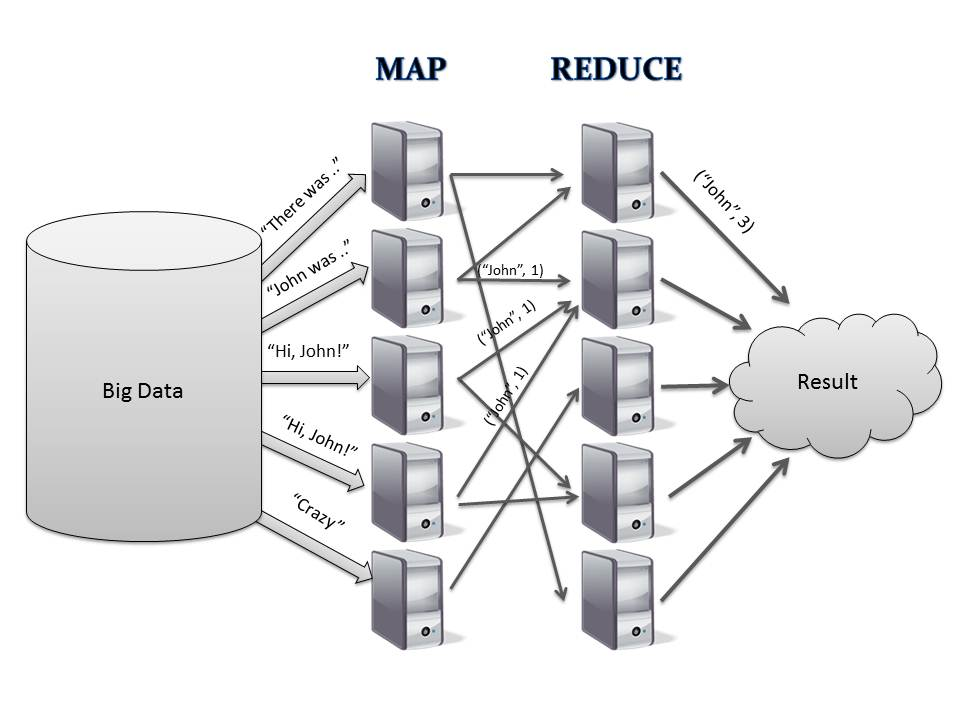
\includegraphics[width=130mm]{figures/mapreduce.jpg}
\caption{MapReduce paradigm}
\label{fig:mapreducepara}
\end{figure}

The popularity of Hadoop's MapReduce framework rises from the fact that many complexities of the system is being handled automatically by the framework. In most typical use cases, the user only needs to provide the method for Mappers and Reducers. Framework will take care of compiling and distributing the code to all of the nodes, and running them in parallel. As previously mentioned it is fault tolerant, it means if during the processing if a task fails, it will restart be restarted, if a node encounters a problem Hadoop will move the computation to another node. It is scalable, which means the program will try to utilize as many nodes as possible based on the size of the input data and amount of available resources, and programmers do not need to concern themselves with that while writing the code. There are also many advanced options that users can do to further optimize the program, but they are generally not required for simple tasks. The other feature of MapReduce and Hadoop in general is that it is available in many different languages. Java, Python, C++, Scala and many more. Figure \ref{fig:mapreducepara} shows the how the word count program will be executed on a cluster.

Newer versions of Hadoop and MapReduce employs more sophistcated Resource manager and Scheduler developed by Vavilapalli et al. \cite{vavila13}. YARN essentially, provides container for running different applications and it is not limited to MapReduce. Spark, Storm and and even simple Java programs can be run on YARN. YARN is more or a less cluster manager program and overviews the resource and allocates resources to different jobs being submitted to it. It has become available as part of Hadoop 2.0 technology Stack.



\textbf{Hadoop Distributed File System (HDFS)}
HDFS is a distributed file system, designed to run on commodity hardware. It provides high throughput access to application data and it fault tolerant. Though initially designed for Hadoop's MapReduce framework, it has been used in many different application.
\begin{figure}[ht!]
\centering
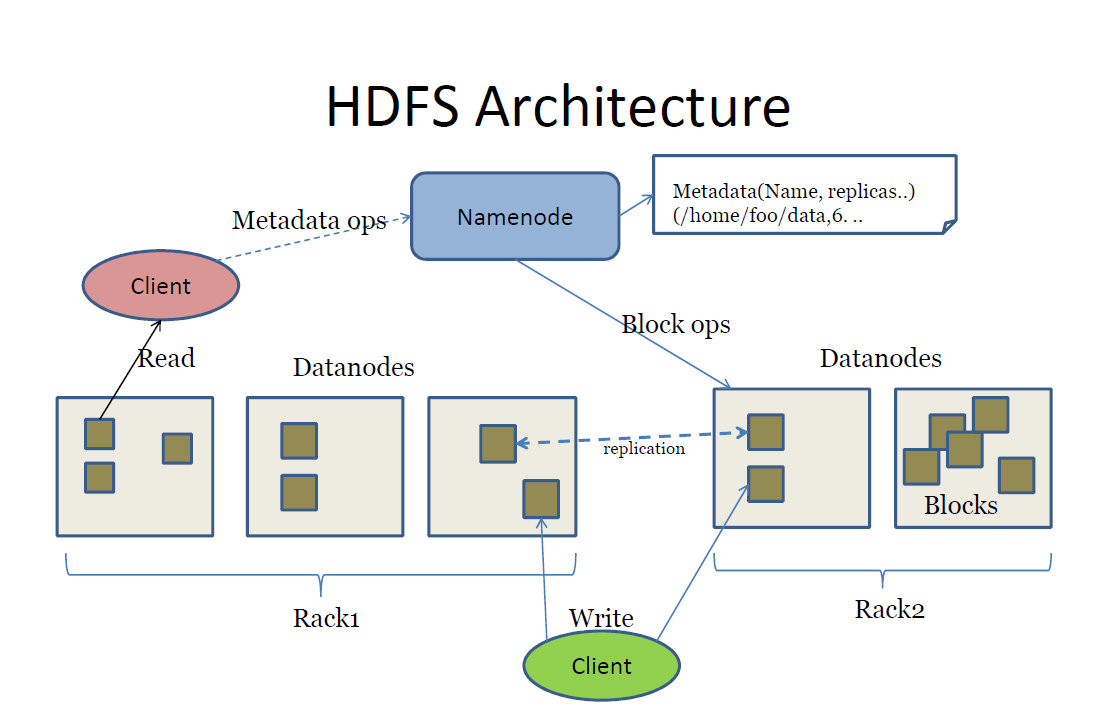
\includegraphics[width=130mm]{figures/hdfsarchitecture.png}
\caption{HDFS Architecture}
\label{fig:hdfsarch}
\end{figure}

It is fault tolerant, meaning if a node in a cluster fails, the data is not gone. HDFS employs a feature called \textit{Data Replication}, which indicates the number of type each object is being replicated. Figure \ref{fig:hdfsarch} shows the high level architecture of HDFS. NameNode keeps track of where are all the same instances of the data is stored and in case a node fails it knows where to look for it. HDFS emphasizes on moving computation is much cheaper than moving data, it is true since HDFS is designed to store BigData sets, Tera or even PetaBytes of data, hence in conjunction with MapReduce, instead of moving the data around, the computation is done on the node containing the data. It is design for high throughput  rather than low latency so it is not ideal for streaming application, although several improvements are being made to further decrease the latency and making it suitable for real time streaming application. Similar to MapReduce it is design to work across heterogeneous hardware and software platforms. Meaning the nodes in the cluster do not have to be identical and even running the same operating system. Hadoop runs on JVM hence it is OS agnostic. 


\subsection{Spark}
Apache Spark \cite{zaharia10} was originally developed in AMPLab at UC Berkeley. The main idea was to solve MapReduce's problems. In contrast to MapReduce's 2 stage program (Map and Reduce), Spark employs an iterative paradigm. It allows users to load data into memory and perform many operations on the data, this is ideal for a lot of Machine learning problems. The underlying frameworks work on entities called Resilient Distributed Datasets (RDDs) \cite{zaharia12}. RDD  is a read only and partitioned collection of data. It can be created from storage or other RDDs. There two types operation on RDDs, transformations and actions. Transformations are operations that will create a new RDD from the existing one, for example \textit{filter}is a transformation operation. The power of RDDs lie in their internal structure, they do not need to be materialized all the time. If a RDD is created using a transformation, it will hold information about how the transformation was made and only apply them to the data once the user requests that through an action or caching the data set. Actions are operations that will materialize the dataset. Users can also ask the RDD to be stored in memory if they know they are going to use its value many times. These characteristics of RDD makes the perfect tool for performing iterative applications. Many machine learning algorithms require iterative calls to the same dataset. This is one of MapReduce's deficiency since every algorithm and job has to be written in terms of Map and Reduces. Spark with the help of RDDs allow many of the well known machine learning algorithms to be applied to without much change to actual algorithm. With success of Spark, it had become part of the Hadoop framework. Recent versions can now on top of Yarn and they have integration with HDFS and other Hadoop components. 
A typical Spark program is consists of a driver program that launches multiple workers. Worker programs are run on data nodes. upon execution of a program, Spark will try to send the computation to where the data is, hence minimizing the network traffic. Spark tracks where the RDDs and their partitions are.
\begin{figure}[ht!]
\centering
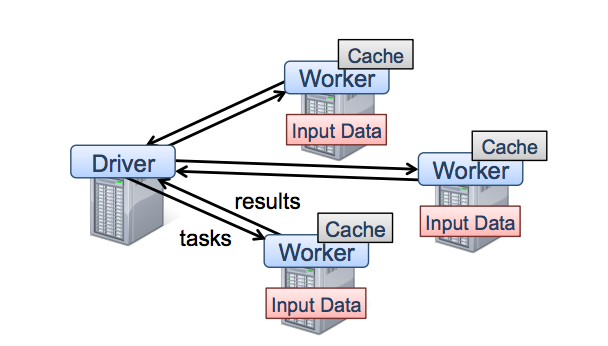
\includegraphics[width=130mm]{figures/sparkprogram.png}
\caption{Spark Program}
\label{fig:sparkprogram}
\end{figure}

User's can control RDDs behavior by persisting it, or caching it. Tests performed on Spark showed that it is 100x times faster than MapReduce and it is able to run application that are not even possible to run using MapReduce. Spark is fault tolerant by means of RDDs. Driver always keeps track the changes made to the RDDs, and they can be recreated from previous stages. So if a node containing some partitions of RDDs is lost they can be recreated using the these information. 
 
\begin{figure}[ht!]
\centering
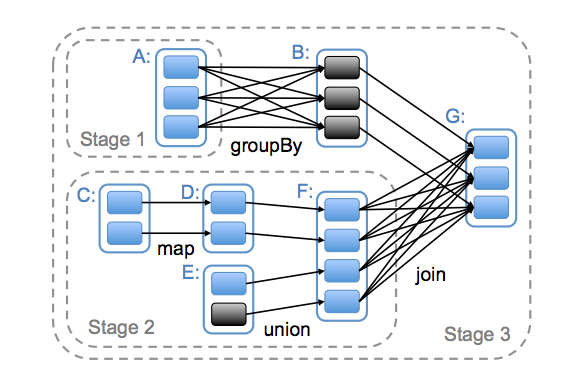
\includegraphics[width=130mm]{figures/rdd.png}
\caption{Spark stages and RDDs}
\label{fig:rdd}
\end{figure}
Figure \ref{fig:rdd} shows how Spark computes job stages. Boxes with solid outlines are RDDs(A, B, ..., G). Partitions are shaded rectangles, in black if they are cached. To run an action on RDD G, the scheduler builds stages at wide dependencies and pipelines narrow transformations inside each stage. In this case, stage 1 does not need to run since B is cached, so we run 2 and then 3. If any of the stages fail, the computation will restart from the last healthy RDD. Also if a node containing some specific partitions of an RDD fails, the RDD will be transferred to another node and the computation will be restarted. 

Spark contains a Machine learning framework named MLib and graph processing framework named GraphX . 
Spark works very well with iterative algorithms, it doesn't have MapReduce limitation which is the result of each job has to be written to disk. Spark has in memory computation which will speed up the process. 
% Spark Word Count Problem in Java and Scala
\newpage

\section{Large Scale Graph Processing Framework}
Large data sets come in many different formats. They are not limited to documents, texts, or key value pairs. One of the more common representation of data is \textit{graphs}. Not only they contain information about individual entities, but graphs also store information about the relationship between these entities. They have been used in many different fields of science to represent data. The most prominent example of a graph data set is the \textit{World Wide Web}, which is a collection of digital pages on Internet and each page may have links to several other pages. In this section, two of the widely used graph frameworks are discussed in detail. Both of these frameworks have been used to implement the methods discussed in section \ref{sec:experiments}. Interestingly, one common computation model used in many of these graph frameworks is based on a model introduced by Valiant \cite{valiant90} called \textit{Bulk Synchronous Parallel} (BSP). A BSP computation model consists of three physical components: 
\begin{itemize}
\item
A component capable of local processing
\item
A network for transferring messages
\item
A hardware which synchronizes the components
\end{itemize}

BSP programs are run in a series of global steps, called \textit{supersteps}. In each superstep, first all nodes run local tasks, and then send messages over the network to other components. Before the next superstep begins, a barrier is set in place that synchronizes all of the nodes and makes sure all the computation and network transfers of the current superstep are finished. Malewicz et al. \cite{malewicz10} developed a system called \textit{Pregel} at Google, which is based on the BSP model and is designed for implementing graph related algorithms. Pregel works by using vertices of the graphs as computation nodes; in each superstep, all vertices performs a local computations, during this phase they only have access to the data internal to the specific vertex which includes the vertex properties and the messages that were sent to the vertex in the previous superstep. After the computation step is done, all vertices may forward a series of messages to other vertices. The messages are usually send through edges, i.e. only vertices connected by an edge communicate with each other, but that is not necessarily the case all the time. Pregel, also takes care of the synchronization barrier and makes sure a new superstep does not begin until the current superstep is finished on all of the vertices.


\subsection{Giraph}
\textit{Apache Giraph} is an iterative graph processing framework, built on top of Apache Hadoop. It is the open source version of Pregel and is now being actively developed by several companies. It is being used in many real case scenarios. For example, Facebook is using it to analyze the graphs formed by users and their connection with their friends. 
In a typical Giraph program, input graph is usually stored and read from the HDFS, once the program starts, Giraph will read the graph and partition the vertices across several nodes. Users can decide how the partition the vertices based on the type of problem they are trying to solve. Giraph by default use a \textit{Hash Partitioner} to partition the vertices. Generally it is a good idea to provide a custom partitioner that works best with the specific problem that is being solved, for example in most of the Giraph programs, in the communication phase, messages are sent along the edges of the graph, so if vertices that are connected to each other are partitioned to the same computation node, the network overhead will be reduced significantly.    
Figure \ref{fig:giraph} shows how computation is done in Giraph .
\begin{figure}[ht!]
\centering
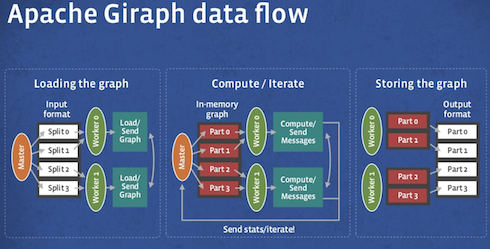
\includegraphics[width=130mm]{figures/giraphdataflow.png}
\caption{Giraph Work Flow}
\label{fig:giraph}
\end{figure}

Each Giraph cluster has a master node and one or more worker nodes. Master node coordinates has the responsibility of reading the graph and partitioning it based on the given partitioner, coordinate the job and the supersteps. Master node is responsible for  all the vertices and making sure that a new superstep does not begin until all the vertices have finished their computation. Each worker node contains several vertices and run the actual program, and coordinate with the master and other nodes through a messages send along the edges or directly to other vertices. Vertices in a Giraph program can be in either of the two states; \textit{Active} or \textit{Not Active}, generally the program continues until all the vertices are Not Active. Vertices themselves are responsible for setting their status after they have finished computing. If a vertex receives a message from other vertices, its state will automatically change to Active.

The figure \ref{fig:sssp} shows supersteps involved with computing the single source shortest path for a simple graph.
\begin{figure}[ht!]
\centering
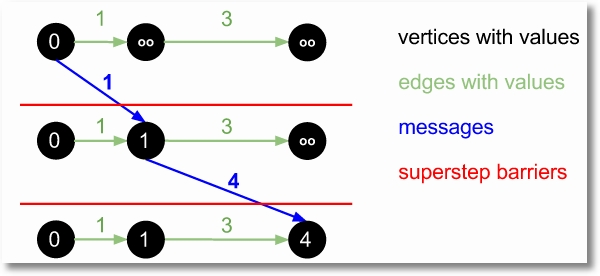
\includegraphics[width=130mm]{figures/giraphsuperstep.jpg}
\caption{Single Source Shortest Path}
\label{fig:sssp}
\end{figure}

The input is a chain graph with three vertices (black) and two edges (green). The values of edges are 1 and 3 respectively. The algorithm computes distances from the leftmost vertex. The initial values of vertices are 0, $\infty$ and $\infty$ (top row). Distance upper bounds are sent as messages (blue), resulting in updates to vertex values (successive rows going down). The execution lasts three supersteps (separated by red lines).

Although Giraph has many advantages over MapReduce, it is still has some limitations, in one Giraph job many iterations can be done, but if graphs should go through several transformation that would require multiple Giraph jobs, which means that the data has be written to HDFS after each job. This adds a lot of IO . A lot of the Machine learning and graph problems are iterative in nature, which will cause Giraph to have severe performance issues in some of these cases. 
% Sample code 
\subsection{GraphX}
\textit{GraphX} is a light API written on top of Spark. It uses the powerfull RDD abstractions as the basis of its computation, by storing vertices and edges in separate RDDs. Similar to Spark, it works well for iterative algorithms and it comes packaged with many of the algorithm such as, PageRank, Label Propagation, Connected Components and ... .  Several important components of GraphX are :
\begin{itemize}
\item VertexRDD: an RDD object consists of a vertex id and a data type. It carries some features in comparison to the traditional RDD, such ensuring vertex ids are unique, optimized joins among different vertex groups. It offers several methods for mapping values, filtering vertices(while preserving their id) and finding difference of two vertex groups.
\item EdgeRDD: similar to VertexRDD, it is a subclass of RDD, which organizes the edges into blocks based on some predefined partitioning strategies. It supports three extra methods; \textit{mapValues} which maps the values while preserving the structure, \textit{reverse} which reverse the edge directions while preserving the attributes, and \textit{innerJoin} which joins two EdgeRDD objects, using the source and destination ids as keys. 
\end{itemize}
The key feature of GraphX comes from the way vertices and edges are stored. GraphX employs different partitioning strategies for storing vertices and edges and while each one have their own advantages and disadvantages, the overall goal is to reduce the amount of communication along edges and have all the vertices close to each other in one computation node to avoid network traffics. The details of GraphX and how it behaves under the hood are beyond the scope of this document. Xin et al. \cite{xin13} described GraphX in detail and GraphX website  \footnote{https://spark.apache.org/graphx/} includes more information about the internal architecture of the system.
GraphX also provides a Pregel like API, that users should only provide the vertex program and the communication strategy. This is one of main advantages of GraphX over Giraph and other similar graph processing frameworks. A GraphX's graph is like any other object in Spark environment, and all the transformations and action available in Spark package can be applied to vertices and edges of the graph. 

Below 
\newpage

\section{Big Data and Network Influence Maximization}
\label{sec:bigdatanetworkinfluelncemaximization}
The original greedy method proposed by Kempe \cite{kempe03} provided a reliable solution to the problem of maximizing influence in network graphs. Several other researchers have worked on finding solutions that find better solutions in terms of accuracy, but most of the researches done in recent years were involved around improving the efficiency of the original method. Leskovec et al. \cite{leskovec07} \textbf{CELF}, Goyal's \cite{goyal112} \textbf{CELF++} and Zhuo et al. \cite{zhuo13} proposed methods that considerably increases the speed of the original Greedy method. Cheng et al. \cite{cheng13} proposed the \textbf{StaticGreedy} method which combined with \textbf{CELF} further improved the speed of the greedy method.  However, non of the proposed methods are scalable and they can only operate on small to medium sized graphs. The bottleneck for the greedy method lies in the function it is trying to optimize.  As discussed in the previous section, the spread function under the Independent Cascade (and Linear Threshold) model cannot be determined exactly due to the edge probabilities. Hence, Monte Carlo method is being used which consists of running the IC model many times(up to 10000 for accurate result) and then averaging over all the simulations. Currently, there are companies and organizations that have graphs of millions to billions of nodes with even more edges, and non of the optimization methods discussed above can be applied to any of these graphs. Even on most powerful clusters running the random process even for one iteration takes a lot of time, essentially rendering the method completely useless. The other group of methods discussed in the previous sections were heuristic methods. They can range from very simple methods such as finding the nodes with highest in or out degree to more sophisticated ones such as \textbf{Single Discount} and \textbf{Degree Discount} discussed by Chen et al. \cite{chen09} or \textbf{SPM} and \textbf{SP1M} proposed by Saito and Kimura \cite{kimura06}. The advantage of heuristic methods are that they are very fast and they can scale to graphs of any sizes, however the accuracy of the solution is not as good as the greedy method. 
\\
In the rest of this section, first the literature on influence maximization for big data and then details of the methods implemented are discussed. Some of methods are fairly simple heuristics and some are based on the methods discussed in previous sections with tweaks that make it possible to implement it on large scale graphs. Changes have to be made to the original algorithms in order to implement the methods using graph frameworks built for processing  large graphs. These frameworks are imposing certain set of restrictions that will make applying some classes of algorithms more difficult. Bulk Synchronous Processing is the base of all the large scale graph frameworks where they are using the method of \textit{Think Like a Vertex}. Although this has many benefits but when it comes to classical IC and LT models, some difficulties will rise. In BSP model, usually algorithms that only need local data are implemented a lot simpler, but in influence maximization we need global access to the network and to find out how many new nodes were affected by adding a node to the initial seed. The whole process is a randomized simulation that should be run hundreds or thousands of time to get a better and more accurate result. Large scale data processing usually suffers in this area, because initializing jobs given huge amount of data whether it is in graph format or others, take up some time and that is something that should be avoided . 
The main challenges when implementing the methods using BSP models are hence, finding ways to avoid the iterative and simulation like implementation and trying to generalize the whole simulation cycle into one BSP job.

While there are many frameworks suitable for extremely large graphs, I have chosen Graphx based on Spark's framework. Its advantage over other frameworks such as Giraph is that it can both implement BSP like and iterative algorithms efficiently. 
\subsection{Monte Carlo Simulation}
On the baseline of most of the methods, lies the \textit{Monte Carlo Simulation}. It represent the Independent Cascade propagation process. Given an initial seed, it will calculate the expected spread, by running the process thousands of times and report the average spread for the initial active set. The distributed method differs from the original implementation in the way the propagation is spread through vertices. In single machine computation, for each vertex in the graph, if the vertex is active it will try to influence all of its neighbors only once and the process continues until no new vertices become active. In distributed implementation, all of the vertices will try to activate their neighbors at once. 
\begin{algorithm}[ht!]
\caption{Monte Carlo Simulation}
\label{alg:simulation}
\floatname{algorithm}{Algorithm}
\begin{algorithmic}
\Require $S$ = initial seed, $R$ = \# of iterations
\State $s_i=0$ for all $0<i<R$
\For {$i$ = 1 to $R$}
	\State $A=S$ 
	\For {each $v \in A$}
		\If {$v_{state} \neq tried$}
			\For {for each $u \in v_{neighbors}$}
				\State try to activate $u$
				\If {$u_{state} = active $}
					\State $A=A\cup \{u\}$
				\EndIf
			\EndFor
			\State $v_{state} = tried$
		\EndIf
	\EndFor
	\State $s_i=|A|$	
\EndFor
\State Output $avg(s)$
\end{algorithmic}
\end{algorithm}
Each vertex carries information about its state. As can be seen from the algorithm, in each iteration of the simulation, every active vertex will try to activate its neighbors, and then change its state to \textit{tried} so it doesn't try to activate again in the next iterations. If a vertex is activated, its state is changed to \textit{active} and it is added to the active set. The process continues until all of the vertices in active set $A$ have tried activating the neighbors and no new vertex is added. The spread of that iteration of the simulation is then stored as the size of the active set $A$ . The final result is the average of all the spreads for every simulation iteration. This is a time consuming procedure because of the number of iterations in the simulation. But this algorithm is not the being used in any of the main methods for finding the initial seeds and it is rather for estimating the spread of a seed. I am only using the procedure to have a baseline of how good an initial seed is and running it even with few number of iterations should give an acceptable estimate.

\subsection{Single Cycle Influence Maximization}
Based on \cite{kempe03} \textbf{Independent Cascade} method, \textit{Single Cycle Influence Maximization} is a simpler and less accurate version of the original algorithm. Implemented using the \textbf{BSP} paradigm, it finds the vertices with maximum influence spread in one iteration, by simulating the Independent Cascade process for all the vertices at once.
\begin{algorithm}[ht!]
\floatname{algorithm}{Algorithm}
\caption{Single Cycle Influence Maximization}
\label{alg:singleccycleIM}
\begin{algorithmic}
\If {superstep == 0}
	\State add your own id to list of influencedBy an increase vertex value by one
	\State try to activate all neighbors by sending its own id
\Else
	\State receive message from every one (message is the id of the vertex)
	\For {each message received}
		\If {it is already in your influencedby list}
			\State vote to halt
		\Else
			\State activate all neighbors by using the message
			\State add to influecedBy list
			\State notify source vertex
			\State vote to halt
		\EndIf	
	\EndFor
\EndIf
\end{algorithmic}
\end{algorithm}
Each vertex contains information about the number of nodes it has affected, and the list of nodes it is affected by. The algorithm is written as point of view of a vertex, that means every vertex executes these steps until the master decides the computation has ended; which either when all of the vertices have voted to halt or a limit for number of iterations is reached. Each vertex sends its own id at the first super step to all of its neighbors, the reason the vertex id is being sent and not just a simple \textbf{Boolean} value is that each vertex has to know who has activated it and store their id and send a message back to them. In the first iteration, when vertices activate their neighbors, any successful activation will be carried on with the affected vertex. For example, if vertex $v_2$ was activated by vertex $v_1$ and now it is trying to activate vertex $v_3$ it will send both its own id $v_2$ and id of the vertex that activated it $v_1$ and subsequently when $v_3$ tries to activate its neighbors it will send its own id as well as $v_1$ and $v_2$. When a vertex is activated it will send a message back to the source of the activation, informing it that it has been activated and the source can now increment its total spread by 1. At the end of the procedure, each vertex has a value indicating its expected spread. The top $k$ vertices are reported as the best initial seed. While this method is fast and performs well on very large graphs it has some draw backs:
\begin{itemize}
\item Activation of a new node is done through only one single random process, based on edge weight.
\item All nodes are trying to activate others, independent of other nodes, depending on network structure this could have some affect on the final result
\item Since each vertex, is sending it's own id and id of vertices that it has been affected by, it might create network traffic.
\end{itemize}

Point one indicates that the result may vary between different runs, because instead other the Monte Carlo Simulation consisting of thousands of iterations, we are only running the simulation once. In the original greedy algorithm, in each iteration one vertex is added the current initial set and the spread is calculated based on the new initial set and the vertex that increases the spread the most is chosen to be added next, but here all of the vertices are operating in silos, disregarding the network effect. Consider an example where two neighbor vertices, individually has the highest spread among all vertices, algorithm \ref{alg:singleccycleIM} will report both of them in the final result, but in reality having two neighboring nodes is not a very good idea, since nodes affected by one are usually affected by the neighbor as well. The last point about network traffic, while in worst case scenarios might be extremely inefficient and in some cases bring the whole cluster down, but that is hardly the case in real big graphs, since first of all most of the big graphs are extremely sparse and the propagation probabilities are so small that a vertex id hardly has to travel more than a few nodes. The idea for this method originates from the observation that Leskovec et al. \cite{leskovec07} made. They have stated, vertices with the best spread in the a iteration of the algorithm usually will have the best spread in the consecutive iterations and in those few occasions that it does it is due the randomness and probability of edges, so in very large scale networks can we simply ignore this fact and just chose the top $k$ nodes by running the algorithm once on the data set . This is of course a very naive implementation . But a good test case, trade of between the quality of the solution and the time it takes to find the `best` solution is an interesting factor here. 

\subsection{Token Based Implementation}
A variation of \textbf{Simple Implementation}method, where the simulation aspect of the \textbf{Independent Cascade} is implemented. In this algorithm, each vertex, instead of trying to activate its neighbors only once, it will try many times. Vertices, will keep many tokens with unique ids. Each token can be tracked back to the vertex it self. In each superstep a vertex will try to activate its neighbors once with every token. If a node is activates using a token, it will notify the original source vertex. The vertex will increment its internal counter for that specific token. Once no new nodes are activated, the program ends and all the vertices will report the average of token counters as their expected spread. Top $k$ nodes then can be selected as the initial seed.
\begin{algorithm}[ht!]
\floatname{algorithm}{Algorithm}
\caption{Token Based Influence Maximization}
\begin{algorithmic}
\If {superstep == 0}
	\State add your own id to list of influencedBy an increase all token counter values by one
	\For{each token}
		\State activate all neighbors using the token
	\EndFor
\Else
	\State receive message from every one (message is the id of the vertex)
	\For {each message received}
		\State extract token out of the message
		\If {token is already in your influencedby list}
			\State vote to halt
		\Else
			\State activate all neighbors by using the token
			\State add to influecedBy token list 
			\State notify source vertex
			\State vote to halt
		\EndIf
		
	\EndFor
\EndIf
\end{algorithmic}
\end{algorithm}
The number of tokens for each vertex determines the accuracy the algorithm, while having thousands of token will basically yield the same result as the actual Monte Carlo Simulation, but in real graphs this is not practical because that means each vertex has to carry a lot of extra information. Choosing the best number of tokens hence is a trade off between a better solution and a faster algorithm. Similar to previous method, depending on the structure of the graph, this method may produce a lot of network overhead, due to the amount of communication that is being done between between nodes. Also it will require a bigger storage since each vertex has to store the spread for many different simulations. So choosing the number of the simulation, not only slows down the process, but it will also increases the risk of a crash in the system, due to size and network overhead.

\subsection{Edge Sampling}
Inspired on \cite{chen09} and \cite{cheng13} method. In \textit{Edge Sampling} method the Independent Cascade process is tackled differently. This method is still using one or a few Monte Carlo Simulations, so in theory it is not as accurate as the Greedy methods, but it can achieve very good results and the number of Simulations can be easily extended as the procedure is very fast. In each iteration of the simulation, instead of having each vertex try to activate its neighbors based on edge probability, a subgraph $G'$ is being sample from the original graph $G$ based on the edge probabilities. Each edge $e$ will remain in the subgraph $G'$ with probability of $e_w$, where $e_w$ is the weight of the edge. $G'$ is now a graph with many unconnected components, in this new graph we can define each vertex $v$'s estimated spread that belong to connected component $C$ as $v_{spread} = C$, the reason for that is since the edges are already sampled by their probabilities, that means any existing edge will definitely propagate the message . Here we can report the top $k$ vertices as the solution. \\
As discussed in Single Cycle Influence Maximization section, one draw back of blindly choosing the vertices with the highest estimated spread was that, vertices that are neighbors or are in the same connected components, will have negative effects on the final spread since having both in the initial seed is redundant, in this method how ever since we know each vertex belongs to which connected components, instead of reporting the top $k$ vertices, we can report one vertex from the top $k$ connected components, that is the connected components with highest number vertices in them. The algorithm can also decrease the noise of the randomness by using many sample subgraphs and averaging the best vertices from all of the samples. The algorithm's definition is presented below.
\begin{algorithm}[ht!]
\caption{Edge Sampling}
\label{alg:edgesampling}
\floatname{algorithm}{Algorithm}
\begin{algorithmic}
\Require $R$ = \# of iterations
\Require $k$ = seed size
\State $v_{total}=0$ for all $v \in G$
\For {$i$ = 1 to $R$}
	\State sample $G'$ from $G$ based on edge probabilities
	\State $C =$ connected components if $G'$
	\For {every vertex $v \in G'$}
       	\State $v_{total} = v_{total} + |C_v|$ where $v \in C_v$
	\EndFor
\EndFor
\For {every vertex $v \in G$}
	\State $v_{spread}=v_{total}/R$
\EndFor
\State Output top $k$ vertices based on their spread
\end{algorithmic}
\end{algorithm}
As with other methods, some modifications have to be made to make this method more suitable in parallel frameworks. The connected components can be efficiently calculated in parallel using \textbf{BSP} model. It is already implemented as part of \textit{GraphX} library. To further optimize the algorithm, changed have been made to the connected component algorithm of \textit{GraphX}. Since for each vertex, we only need the size of the its corresponding connected component, we can modify the original algorithm to instead of reporting the connected component id, it will report the size of the connected component. The result of the new connected component algorithm would then be the list of vertices, each vertex carrying its id and corresponding connected components size. In this method, the connected component size is equal to the expected spread for each algorithm. The algorithm starts by initializing the list of all vertices. Every vertex's expected spread is 0 at the beginning. In each iteration of the simulation, the sizes are updated based on component size. The update can be done simply by doing a join. Vertex joins are very efficient in \textit{GraphX}, can be done very quickly. Increasing the number of simulations will increase the accuracy, but it also slows down the process. In the next sections, these trade offs will be discussed and the result of the algorithm will be presented.

\subsection{Degree Discount Heuristic}
\label{subsec:degreediscount}
In previous section, Chen et al. \cite{chen09} heuristic for choosing the best vertices for initial seed were discussed. Their method has several advantages that make it easy to implement, and very fast and scalable. This method does not require a simulation as it is a simple heuristic based on the degree of each vertex. According to Chen et al. it yields an extremely good result which is in par with greedy methods. Since the method is simply working vertices individually it is ideal for a BSP graph framework. 
\begin{algorithm}[ht!]
\floatname{algorithm}{Algorithm}
\caption{Degree Discount}
\label{alg:degreedicount}
\begin{algorithmic}
\State $S=\emptyset$
\For{each vertex $v$}
	\State compute its degree $d_v$
 	\State $dd_v=d_v$
 	\State $t_v = 0$
\EndFor
\For{$i$ = 1 to $k$}
	\State $u = \argmax_v \{dd_v |  v \in V \ S\}$
	\State $S = S \cup \{u\}$
	\For{each neighbor $v$ of $u$ and $v \in V\ S$ }
		\State $t_v = t_v + 1$
		\State $dd_v = d_v - 2t_v - (d_v - t_v)t_v p)$
	\EndFor
\EndFor
\State output $S$
\end{algorithmic}
\end{algorithm}
Compared to other heuristic methods that will be discussed in the next section, this method is more difficult to implement in a \textbf{BSP} model. The number of iterations the algorithm runs depends on the seed size. Basically, after initializing all the vertices, in each iteration the best vertex is chosen and added to the seed set. After that, the values for the neighbors of the selected vertex will be changed based on the formula presented in the algorithm. This means for a seed set of size $k$, the algorithm runs for $k$ iterations. This will make the implementation in \textbf{BSP} a bit more difficult. But with \textit{GraphX} the state of the graph can be easily tracked, local changes can efficiently be applied. Hence the time complexity of the algorithm is linear and it increases linearly with the number of expected seeds

\subsection{Other Heuristics}
\textbf{Random}: $k$ Random vertices are selected as the solution. This is used as a baseline for other methods to see if they perform better than just choosing nodes at random. \\
\textbf{Degree}: Degree of a vertex is defined as the number of edges connected to a vertex. In this method, the vertices with the highest degree are chosen as the initial seed. \\ 
\textbf{Single Discount}: Improved version of Degree heuristic. After a vertex is chosen as the seed, it is removed from the graph, that means all of its neighbors' degree are reduced by one. This yields a better result that Degree heuristic, since it lower the chance of neighboring vertices to be selected as the initial seed. \\ 
\textbf {Page Rank} : Based on the popular Page Rank algorithm \cite{page99}, the algorithm was originally used in Google's search engine, to rank websites based on their importance. 

\newpage


\section{Experiments} \label{sec:experiments}
In this section all the experiments are explained in details. Experiments include the methods and the data sets described in the previous sections. 
\subsection{Experiment Setup}
Experiments are run on two different computation platform. For smaller data set, to test the accuracy and speed of the methods the experiments are run on a single machine. Bigger data sets are run on an EMR cluster. The details are below. 

\begin{itemize}
\item Single node setup : \\
A Macbook Pro with 2,4 GHz Intel Core i5 processor and 8 GB of memory. 
\item Cluster setup: \\
5 m3.xlarge Amazon EMR nodes. Each node has 4 CPU cores, 15 GB of memory and 80 GB of SSD storage.
\end{itemize}
Except for the Greedy CELF method, which is implemented in a single threaded Java application, the rest of methods and the simulation are implemented using Apache Spark version 1.3.0 in Scala language. 


\subsection{Data set}
Below is an overview of the data sets used in the experiments. All of the data sets are provided an an edge list format. In each line there are two vertices id separated by a tab character. The two vertices are end points of an edge. 
\subsubsection{ArXiv collaboration network data set}
Two data sets from the e-print arXiv is chosen for testing. Same two data sets have been used in \cite{kempe03} and \cite{chen09}. The data set contains academic collaboration for scientific research papers. In this data set, vertices represent researchers and edges define a collaboration between two researchers on writing a scientific paper. Two data sets have been chosen, they have been used by several other researchers in the field of influence maximization and can provide a good comparison for the quality of the methods. The data sets are small comparing to the data sets currently considered as Big Data, but since there aren't many previous research done in Big Data, the \textit{High Energy Physics-Theory} graph, which contains papers from 1991 to 2003, with 15,233 nodes and 58,981 edges is used as a base comparison of the methods proposed in section \ref{sec:bigdatanetworkinfluelncemaximization} and state of the art greedy methods.
The data sets in graph formats were made available for public by \cite{chen09}. It can be found at http://research.microsoft.com/en-us/people/weic/graphdata.zip. It is in Edge List Format where each line of the file, contains two values the first on is the source and the second one is the destination of an edge.

\subsubsection{LiveJournal Social Network}
LiveJournal is a free online community with almost 10 million members, with many of them being active . Similar to other types of social networks, users can form friendship with other members. It consists for 4,847,571 vertices and 68,993,773 edges. Considerably larger than a lot of data sets usually used in influence maximization research, but still not at the same scale as current big data sets used in research and industry.  It is also available in \textbf{Edge List Format} format.

\subsection{Methods \& Implementation details}
List of influence propagation methods used in the experiments
\begin{itemize}
\item \textbf{Single Cycle}: Based on \textit{Single Cycle Influence Maximization} algorithm. This method is implemented using \textit{Apache Giraph} for ease of implementation.
\item \textbf{Multi-attempt Single Cycle}: Based on \textit{Token Based Influence Maximization} algorithm. Similar to single cycle, this method is also implemented in \textit{Apache Giraph}
\item \textbf{PageRank}: Based on popular \textit{Page rank} algorithm developed by Google. Implemented using \textit{Spark's Graphx}.
\item \textbf{Degree}: Simple method, that chooses nodes with highest degree. Implemented using \textit{Spark's Graphx}.
\item \textbf{Degree Discount}: Based on \textit{Degree Discount} heuristic, discussed in previous section. This method is also implemented using \textit{Spark's Graphx}.
\item \textbf{Edge Sampling}: Based on \textit{Edge Sampling}algorithm, this method is implemented using \textit{Spark's Graphx}.
\item \textbf{Random}: Choose initial seed randomly. This is used as base comparison. 
\end{itemize}

Some of the methods proved to be easier to implement using certain framework. There are subtle differences between, Graphx's pregel API and Giraph's pregel API. Giraphx's pregel requires the user to supply three methods : 
\begin{itemize}
\item Vertex program : Responsible for modifying the value of vertices. It receives the messages for each vertex and run them separately for each vertex. The return type, is the same as the vertex data type and cannot be changed.
\item Send message : Inputs an \textit{EdgeTriplet} data type, which contains the source, and destination vertices along with their attributes, and edge data type. It returns an \textit{Iterator} which specifies the message and the destination the message should be send to.
\item Merge messages: Merge messages intended for a destination vertex. It receives two messages of the same type and return the combined message that should have the same data type as the input messages.
\end{itemize}

Although, these three methods work along side each other, they are separated and do not have access to the internal values of each other. This makes it very difficult and non efficient to implements some of methods, for example: Single Cycle and Multi-attemp Single Cycle. These two algorithm, are designed to act upon the message they receive immediately and based on value of each message, they have to decide either to send a message to neighboring vertices or not. This is unfortunately not possible in Graphx. \\
Giraph's pregel API is designed differently. It consists of the following methods, some of which are optional and do not need to be supplied by the user :
\begin{itemize}
\item compute : The most important method. It has to be supplied by the user. The input to the method, is the vertex and all messages intended for that vertex. User can modify the value of vertex, send messages to other vertices , and etc .
\item initialize : Called once at the beginning of the program. Generally used, for defining any aggregators or other global operations that will be used during the run time of the program.
\item preSuperStep : Called before every super step. It is not mandatory, but it is generally used to update global values before the super step begins.
\item postSuperStep: Similar to previous method, with the difference that it is run after super step has ended.
\item sendMessage: Method for sending messages to other vertices. It requires the id of the destination vertex and the intended message. This method is generally not overridden, and it is simply intended to send a message to another vertex. It can be called many times from the compute method. Giraph takes care of synchronization process, generally all the messages are send once all the compute methods for all the vertices are executed.
\end{itemize}

Giraph provides more freedom to run algorithms in pregel framework, as it leaves the responsibility of sending messages to the user rather than enforcing it to be send in every iteration. This makes, Giraph ideal for implementing the first two methods, because the decision to either send or not send a message depends on the content of the message itself.


\section{Results and Discussions}
In this section, the results of running the algorithm discussed in section \ref{sec:bigdatanetworkinfluelncemaximization} are shown. The spread and running time of different methods on different real graphs are and reported. In the last part of the section, several random graphs having common characteristics found in real graphs are used to further analyze and explain the advantages and disadvantages of each of these methods.

\subsection{ArXiv collaboration network data set} 
In this section the result of running different methods on collaboration network data set are explained. To calculate the spread for each method, multiple simulations needed to be run, in these set of experiments number of simulations is set 100. While increasing the number will make the result more accurate, but it will also increase the running time. Experiments have been run with different number of simulations and the results show that the difference between number of simulations is not very significant. 
\begin{figure}[ht!]
\centering
\includegraphics[width=100mm]{figures/hep/searchmethods.png}
\caption{Search methods}
\label{hep:searchmethods}
\end{figure}
Figure \ref{hep:searchmethods} shows the result of running search methods on collaboration graph. Clearly the greedy method is much better than all of the other methods. As discussed in previous chapters, the underlying approach of the other three methods are similar and hence their spread is more or the less the same. Both edge sampling's number of iterations and multicycle's number of tokens are set to 100, and their results are a little better than single cycle, but as explained earlier both the noise from calculating the spread and the algorithms themselves make it difficult to clearly distinguish their differences.
\begin{figure}[ht!]
\centering
\includegraphics[width=100mm]{figures/hep/heuristicsmethods.png}
\caption{Heuristic methods}
\label{hep:heuristicmethods}
\end{figure}
Figure \ref{hep:heuristicmethods} shows the spread of the heuristics methods on collaboration network graph.  All heuristics methods expects random produce similar results. Page rank is slightly better than degree and degree discount method, mostly because when calculating the importance of a vertex, it doesn't just consider its immediate neighbors. Comparing heuristics with search methods shows that greedy methods is the best among all of the methods. Heuristics methods are performing better than edge sampling, single and multi cycle methods. In the last part of this section, several artificial graphs are generated each one having different graph properties such as skewness and sparsity, for each of the graphs, the heuristic methods and edge sampling are run in order to study the effectiveness of each method on different types of graphs.

\begin{table}[ht!]
\centering
\begin{tabular}{ |c|c| }
\hline 
  method & time (s)\\
  \hline 
  random & 0.84\\
  degree & 1.01\\
  degreediscount&1.156\\
  pagerank&2.338\\
  edgesampling&7.73\\
  singlecycle&45.2\\
  multicycle&50.34\\
  \hline 
\end{tabular}
\caption{Running time}
\label{hep:timetable}
\end{table}
Table \ref{hep:timetable} shows the running time all of the methods expect for greedy. As explained in previous chapters, running time of all of the methods specified in the table is independent of seed size, that is the biggest advantage of these methods over the greedy method. Figure \ref{hep:times} shows the running time of the greedy method based on input size, to make the comparison easier, running time of other methods are also shown in the figure. To find a seed set of size 100 on the collaboration network data set after applying the celf optimization, it takes almost 2 hours, and this graph is much smaller than a typical big data graph. Being a NP-Hard problem, the algorithm will not scale linearly, this means for data sets that are 100 times bigger than collaboration network, it might take thousands of time more to run the algorithm
\begin{figure}[H]
\centering
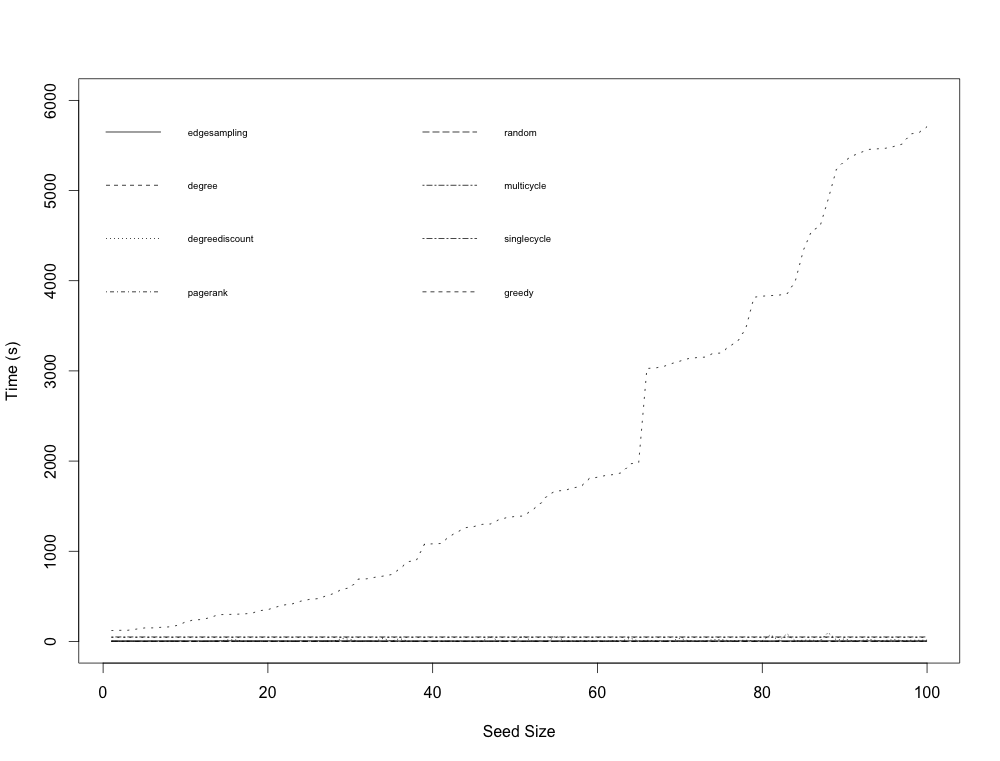
\includegraphics[width=130mm]{figures/hep/times.png}
\caption{Running time of different methods on collaboration network data set}
\label{hep:times}
\end{figure}

\subsection{Live Journal}

\begin{figure}[ht!]
\centering
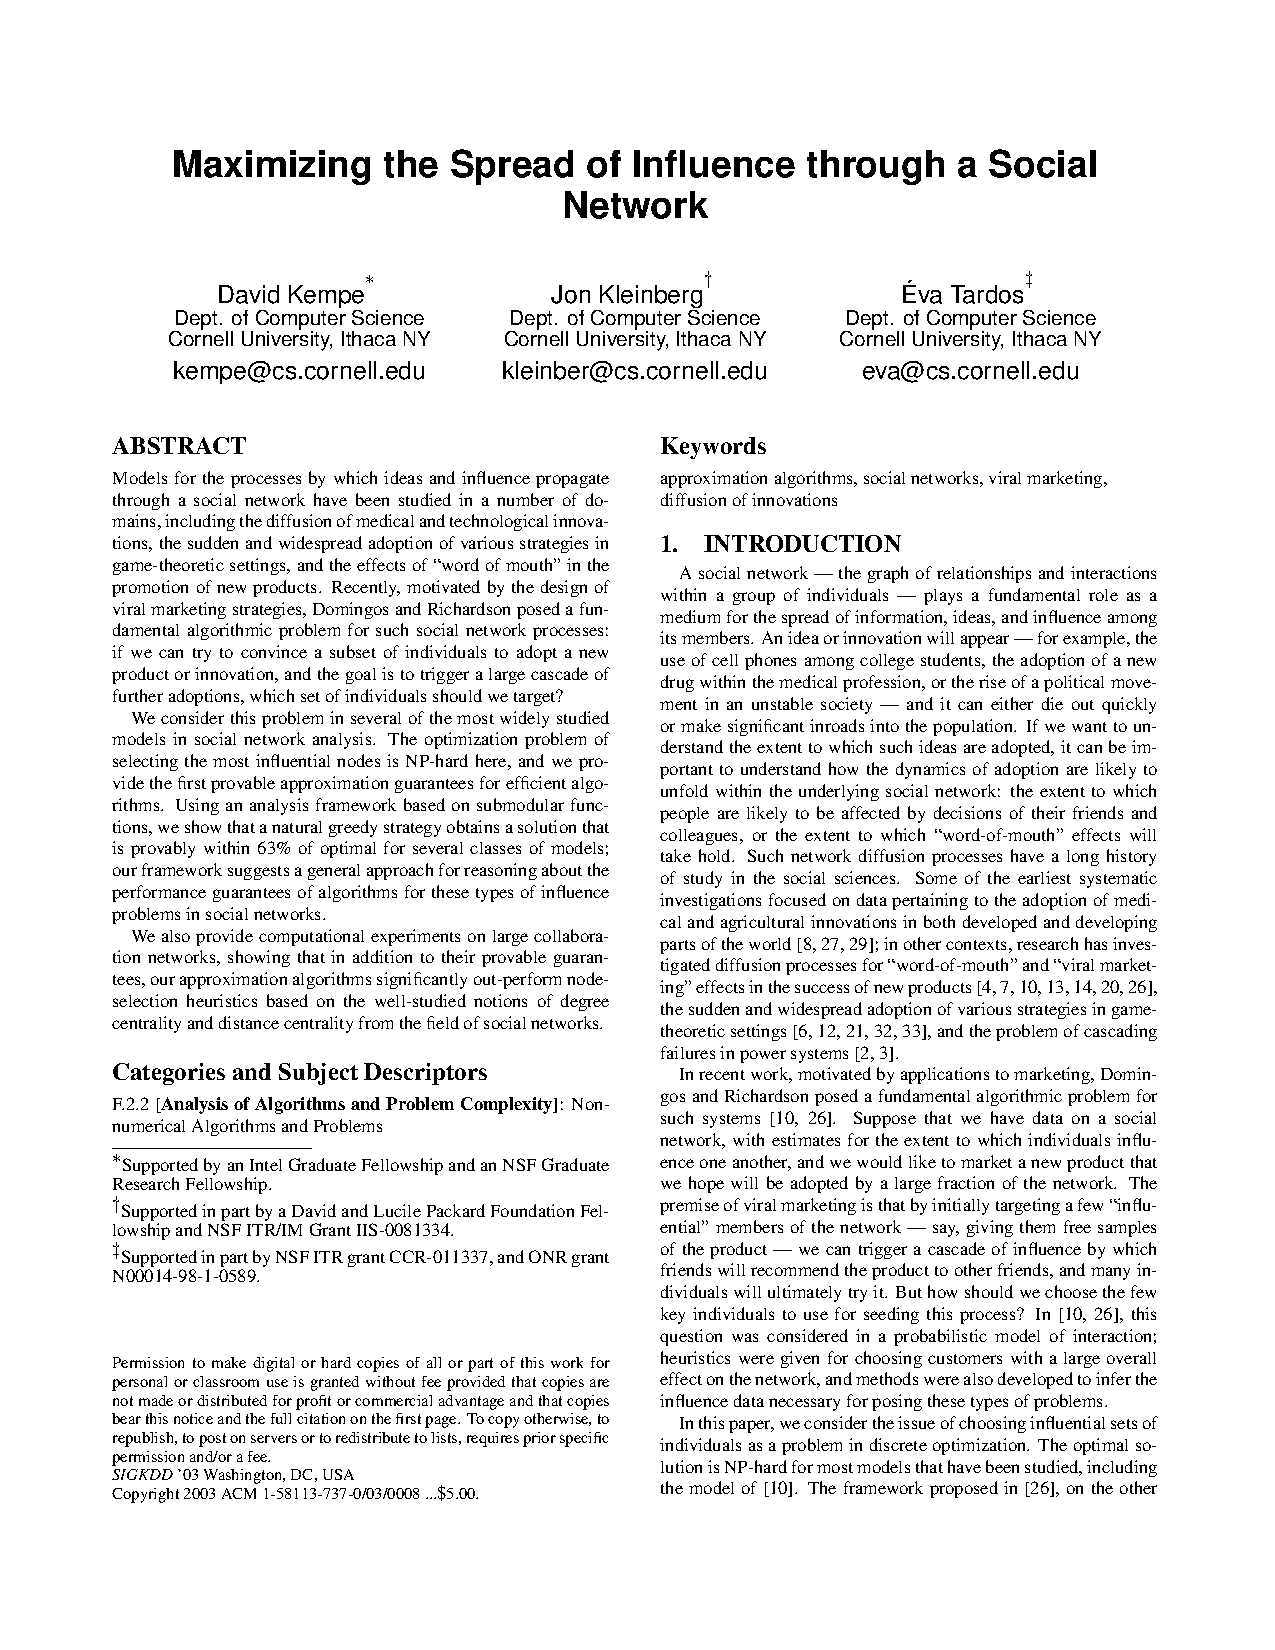
\includegraphics[width=130mm]{figures/journal/spread.png}
\caption{Spread of different methods on Live Journal Data set}
\label{journal:spread}
\end{figure}

Same as collaboration network data set, the number of simulations is set to 100. Here the seed sizes are much larger, and the results are reported for seed sizes of 10000, 20000, 30000, 40000 and 50000. Due to its size, running the greedy method is impossible, and both the single cycle and multi cycle as specified earlier run into problems because of the massive amount of data they have to store in memory. For this data set, only edge sampling, degree, page rank and random seed selection methods are executed and the results are reported below.
Figure \ref{journal:spread} shows the spread achieved by running different methods on the live journal data set. Horizontal axis shows the seed size, and the vertical axis shows the total spread. From the figure it is clearly obvious that page rank and edge sampling are superior to the other methods. Random method is just used as a baseline to compare with the other methods. The figure shows that the same algorithms behave differently on different graphs. In the next section this will be studied in more detail.

\begin{table}[ht!]
\centering
\begin{tabular}{ |c|c| }
\hline 
  method & time (s)\\
  \hline 
  random & 21\\
  degree & 49\\
  pagerank&206\\
  edgesampling&705\\
  \hline 
\end{tabular}
\caption{Running time}
\label{journal:time}
\end{table}

Table \ref{journal:time} shows the running time of different algorithms. Random and degree methods as expected are very fast, page rank and edge sampling both run in acceptable time given the input size. As explained earlier, greedy method cannot scale to graphs of these sizes. 

\pagebreak
\pagebreak


\subsection{Artificial Graphs}
In this section the spread of degree, pagerank and edge sampling methods on different types of artificially generated graphs are investigated. As a baseline the spread of random set of seeds are also drawn. Each of the graphs bear some specific properties that distinguished graphs from each other. As observed from the real graph examples in the previous sections, edge sampling method is not always performing better than the heuristics methods such as pagerank and degree. Here it will be shown for which types of graphs edge sampling method is performing better. 
\begin{figure}[ht!]
\centering
\includegraphics[width=130mm]{figures/artificial/random.png}
\caption{Random graph of 1000 vertices and 4000 edges}
\label{art:random}
\end{figure}

Figure \ref{art:random} shows the spread on a graph with randomly generated edges. The source and destination of edges are sampled randomly from all the vertices available. From the figure, it can be observed that pagerank and degree method are performing better than edge sampling, although the difference in the final result is not significant. 

\begin{figure}[ht!]
\centering
\includegraphics[width=130mm]{figures/artificial/sparse.png}
\caption{Sparse graph with 1000 vertices and 1000 edges}
\label{art:sparse}
\end{figure}

Figure \ref{art:sparse} shows the spread on a sparse graph. The graph is generated similar to random but with a lot fewer edges. Similar to the random graphs, the spread of the different methods do not differ significantly.

\begin{figure}[ht!]
\centering
\includegraphics[width=130mm]{figures/artificial/skewed.png}
\caption{Skewed graph with 1000 vertices and 4000 edges}
\label{art:skewed}
\end{figure}

Figure \ref{art:skewed} shows the spread on a skewed graph. Here the difference in the results are more significant. As expected page rank and degree method are performing better than edge sampling. This can be explained by the fact that seeds are picked from the more dense regions of the graph and page rank and degree can are choosing the nodes with highest amount of neighbors. Due to the nature of edge sampling methods, it is possible that some nodes from the less denser area of the graph are chosen as seed which have caused the spread for edge sampling method to be lower.

\begin{figure}[ht!]
\centering
\includegraphics[width=130mm]{figures/artificial/clustered.png}
\caption{Clustered graph with 1000 vertices and 10000 edges}
\label{art:clustered}
\end{figure}

The vertices and edges in the graph of figure \ref{art:clustered} are clustered into two set. The smaller cluster is a fully connected component, which means all of the vertices are connected to each other. Because of this all of the vertices from the smaller cluster have very high degree. This explains the reason why degree method is not performing as well as edge sampling and page rank methods, both of which consider more global information when choosing the seeds.\\
\subsection{Discussion}
From these experiments performed in this section, it is obvious that while none of the methods are performing as good as the greedy method, some of them are good candidates for influence maximization on large graphs. Pagerank, Degree and Edge Sampling methods are very fast, and the spread achieved by these methods are acceptable. Different properties of graphs, affect the performance of each of the methods, hence the best way to chose the seed is to run all three methods on the graph and compare the spread for different seed sizes. None of the methods depend on the seed size, and running them once will return the list of vertices in order of how good they are in increasing the spread in the graph. Users then can easily chose the desired number of seeds.

\pagebreak
\section{Conclusion}
In this document, the problem of influence maximization was discussed. One of the main issues in solutions to problem is the scalability. Due to the nature of the solutions proposed, none can perform well for large scale graphs. Over the past decade, with wide spread usage of internet data collection has been the focus of many big firms. Social networks and online store are gathering data about millions of users everyday. The information about users are stored in graph data structures that sometimes consists of millions (even billions) of nodes and  many more edges. Applying some of the solutions proposed for influence maximization to graphs of these scales are impossible and even on the strongest super computers will take days or even months to see the result. Here, I have identified why the solutions are not scalable and proposed some new or modified solutions to work with graphs of this scale. Several frameworks for processing large scale data have been created over the past couple of years, most notably are Hadoop and Spark. Both of which are designed to run on commodity computers, and are highly scalable. They both have a built in frameworks for processing graphs; Giraph which is on top of Hadoop and Graphx on top of Spark. Methods described in this document, are implemented using these two frameworks. In last section, several experiments on different data sets were performed and the results were presented. \\
Theoretically, it was proven by \cite{kempe03} that the greedy method provides the best solution to the influence maximization problem, but the inefficiency of the method for some types of graphs excels its quality and justifies the sacrifice of quality for performance. Several of the methods discussed here, run very fast and they are not affected by the size of the input graph. In some of the data sets that it was possible to run the greedy methods, some of these scalable methods provided comparable solution in term of quality with the greedy algorithm, and result showed that even on small data sets, greedy method will take extremely long amount of time, making it virtually impossible to run the greedy method on large scale graphs that are very common today. \\
Influence maximization is very large topic and in this paper only the basic problem was covered. Several challenges were left out of this thesis, and many other challenges still remains. Finding a more deterministic function or a probabilistic function that does not rely on the Monte Carlo simulation is one of the areas that has been and still being studied. Topic based influence maximization, i.e. users influencing each other differently with regards to different topics is another area that was not covered in the thesis. Influence degradation, is also another interesting topic that involves dynamic influence probabilities that will change with time are some of the other interesting areas that worth exploring.

\pagebreak



\bibliographystyle{tktl}
\bibliography{bibliography}
\lastpage
\appendices
\pagestyle{empty}
\end{document}


